\chapter{Architektura sprzętowa i analiza dokumentacji technicznej}
\label{chap:analiza_sprzetu}

\section{Opis stanowiska badawczego}
% Wprowadzenie do zrealizowanej wcześniej części sprzętowej (PCB, obudowa).
Stanowisko badawcze ma formę autonomicznej, trójmodułowej obciążnicy pasywnej prądu stałego, umożliwiającej skokową regulację pobieranej mocy. Architektura fizyczna urządzenia została zaprojektowana z uwzględnieniem separacji obwodów silnoprądowych od układów cyfrowego sterowania. Cały system składa się z następujących głównych bloków:

\begin{itemize}
	\item \textbf{Tor główny:} Badane źródło zasilania podłączane jest za pomocą zacisków bananowych z lewej strony obudowy. Jest ono izolowane i zabezpieczane od reszty układu poprzez styczniki GIGAVAC.
	
	\item \textbf{Moduły wykonawcze:} Każdy z trzech modułów wyposażony jest we własny radiator z rezystorami mocy. Układ został wyposażony w wentylatory do chłodzenia powietrznego, zamontowane od dołu bloku rezystorów oraz termistory NTC do pomiaru temperatury. Uzupełnieniem chłodzenia całego systemu są dwa wentylatory umieszczone na górze obudowy.
	
	\item \textbf{Układ kondycjonowania sygnałów i przełączania:} Płyta przekaźników sterujących stanowi interfejs między mikrokontrolerem a torem mocy. Znajdują się na niej przetworniki prądu i napięcia umożliwiające akwizycję tych wielkości do postaci cyfrowej. Ponadto, płyta ta zawiera przekaźniki zmieniające konfigurację połączenia rezystorów mocy w celu zmiany obciążenia oraz dedykowany przekaźnik wysterowujący główne styczniki próżniowe GIGAVAC.
	
	\item \textbf{Jednostka centralna:} Algorytmy sterowania oraz maszyna stanów realizowane są przez główną płytę cyfrową, której sercem jest procesor sygnałowy Texas Instruments TMS320F28069.
	
	\item \textbf{Zasilanie pomocnicze:}  Energia niezbędna do zasilania elektroniki, cewek przekaźników oraz wentylatorów dostarczana jest z pokładowego zasilacza LRS-75-24, który zasilany jest z napięcia sieciowego zabezpieczonego bezpiecznikiem nadprądowym EATON o charakterystyce B6. Zasilacz znamionowo dostarcza napięcie 24V oraz prąd 3.2A
	
	\item \textbf{Lokalny interfejs użytkownika (HMI):} Panel przedni urządzenia umożliwia pracę stanowiska bez udziału komputera nadrzędnego. Wyposażono go w wyświetlacz alfanumeryczny, sygnalizacyjne diody LED oraz przełączniki dwu- i trójpozycyjne służące do ręcznego ustalania trybu pracy i konfiguracji obciążenia. Komunikację z systemami zewnętrznymi umożliwiają dwa porty DB9 których głównym zadaniem jest obsługa magistrali CAN. Panel przedni posiada również port USB-B służący do programowania mikrokontrolera.
\end{itemize}

Architekturę sprzętową stanowiska zilustrowano na schemacie blokowym (Rysunek \ref{fig:schemat_blokowy}).

% Tutaj wstawisz wygenerowany z Draw.io schemat blokowy
 \begin{figure}[htb]
	     \centering
	     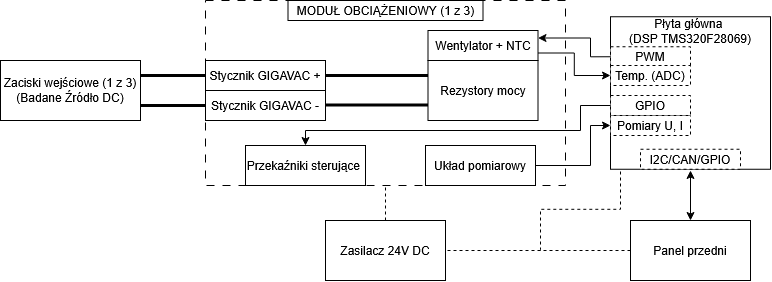
\includegraphics[width=\textwidth]{rysunki/schemat_blokowy_obciaznicy}
	     \caption{Schemat blokowy obciążnicy pasywnej z uwzględnieniem jednego modułu wykonawczego}
	     \label{fig:schemat_blokowy}
	 \end{figure}



\section{Mikrokontroler TMS320F28069}
% Analiza noty katalogowej rodziny C2000 i peryferiów użytych w projekcie (ADC, ePWM, eCAN).

\section{Moduły wykonawcze i styczniki GIGAVAC}
% Opis układu załączania obciążeń (rezystory 5.5/22/88 omów) i parametrów styczników.

\section{Układy pomiarowe i sensoryka}
% Pomiary napięć, prądów, czujniki NTC oraz izolacja galwaniczna układu.